\section{Clock}

Embora o tempo físico seja contínuo, sistemas digitais operam a partir de amostragens discretas desse domínio. Nesse contexto, a evolução do sistema é modelada como uma sequência de estados indexados por instantes discretos $t \in \mathbb{N}$.

Como descrito na seção \textbf{\nameref{sec:cronometro}}, o cronômetro, enquanto uma Máquina de Estados Finita (FSM), possui seu estado definido pela tupla $(H_t, M_t, S_t, D_t)$ no instante $t$.

Para que essa modelagem discreta seja consistente com o comportamento físico do circuito, é necessário um mecanismo que determine de forma precisa quando as transições de estado devem ocorrer.

O clock cumpre esse papel, atuando como uma referência temporal global que define os instantes de amostragem do sistema e sincroniza todos os seus componentes.

O clock impõe uma ordem temporal ao sistema, evitando transições concorrentes e garantindo que a função de transição $\delta$ seja aplicada de forma determinística:

\[
S_t \xrightarrow{\delta} S_{t+1}
\]

sem ambiguidades causadas por atrasos de propagação nos componentes lógicos.

Trata-se de um sinal periódico que alterna entre níveis lógicos alto (1) e baixo (0), estabelecendo uma estrutura temporal comum para o circuito. 

\begin{figure}[htbp]
    \centering
    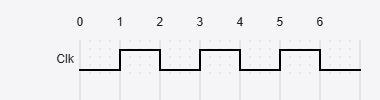
\includegraphics[width=0.7\linewidth]{images/clock-waveform.png}
    \caption{Onda de clock}
    \label{fig:clock-waveform}
\end{figure}

\subsection{Propriedades do Clock}

Formalmente, um sinal de clock pode ser modelado como uma função periódica discreta ou contínua no tempo. No contexto físico, considera-se inicialmente uma representação contínua:

\[
clk : \mathbb{R}_{\geq 0} \to \{0,1\}
\]

tal que:

\[
clk(t + T) = clk(t)
\]

onde \(T > 0\) representa o período do sinal.

A frequência do clock é definida como o inverso do período:

\[
f = \frac{1}{T}
\]

Em sistemas digitais síncronos, o clock estabelece os instantes nos quais os elementos de memória amostram suas entradas e atualizam seus estados internos. Dessa forma, embora o sinal físico exista continuamente no tempo, a evolução lógica do sistema ocorre apenas em instantes discretos:

\[
t_n = nT, \quad n \in \mathbb{N}
\]


Assim, o período \(T\) pode ser decomposto em dois intervalos:

\[
T = t_{high} + t_{low}
\]

onde:

\begin{itemize}
    \item \(t_{high}\): duração do nível lógico alto;
    \item \(t_{low}\): duração do nível lógico baixo.
\end{itemize}

A razão entre o tempo em nível alto e o período total define o \textit{duty cycle} $D$ do sinal:

\[
D = \frac{t_{high}}{T}
\]

Esse parâmetro é relevante em circuitos sensíveis à largura temporal dos pulsos.

\begin{figure}[H]
    \centering
    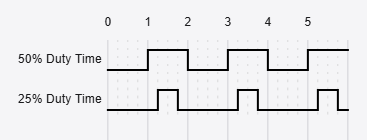
\includegraphics[width=0.7\linewidth]{images/duty-cycles.png}
    \caption{Exemplos de duty cycle}
    \label{fig:duty-cycles}
\end{figure}

Além disso, sendo um sinal periódico, o clock pode ser descrito por uma fase instantânea \(\theta(t)\), que representa sua posição relativa dentro de um ciclo.

Matematicamente:

\[
\theta(t) = 2\pi \frac{t \bmod T}{T}
\]

com:

\[
\theta(t) \in [0, 2\pi)
\]

A fase fornece uma representação contínua da evolução temporal do sinal ao longo de um período.

Embora sistemas digitais normalmente não utilizem diretamente o valor contínuo da fase, eventos específicos associados a ela possuem importância fundamental. Em particular:

\begin{itemize}
    \item \(\theta = 0\): borda de subida;
    \item \(\theta = \pi\): borda de descida.
\end{itemize}

Essas transições definem os instantes nos quais máquinas de estado e elementos sequenciais realizam atualizações sincronizadas.

A modelagem em termos de fase também é útil para a análise de fenômenos temporais como:

\begin{itemize}
    \item \textit{skew}: desalinhamento temporal do clock entre diferentes regiões do circuito;
    \item \textit{jitter}: variações temporais na periodicidade do sinal.
\end{itemize}

Assim, um sinal de clock periódico pode ser caracterizado de forma compacta, pela tupla de parâmetros:

\[
(T, D, \theta_0)
\]
\subsection{Atraso de Propagação em Circuitos}

Em circuitos digitais reais, as transições de sinal não ocorrem de forma instantânea. Cada elemento lógico introduz um atraso entre a aplicação de uma entrada e a estabilização da saída, denominado atraso de propagação ($t_p$).

Como consequência, diferentes partes do circuito podem, temporariamente, operar sobre valores inconsistentes de um mesmo sinal. Em circuitos com realimentação, esse fenômeno pode levar a oscilações ou transições espúrias.

O uso de um sinal de clock mitiga esse problema ao restringir as mudanças de estado a instantes discretos, nos quais se assume que os sinais já se estabilizaram.

Considere um circuito combinacional que implementa uma função booleana $f : X \rightarrow Y$. Em um modelo ideal, a saída $y \in Y$ é dada por:

\[
y(t) = f(x(t))
\]

Em um circuito físico, entretanto, a resposta da saída é retardada pelo atraso de propagação. Um modelo temporal mais realista é dado por:

\[
y(t + t_p) = f(x(t))
\]

ou, de forma equivalente,

\[
y(t) = f(x(t - t_p))
\]

Essas expressões indicam que a saída em um dado instante depende de valores passados da entrada, refletindo o comportamento causal do sistema físico.

Esta problemática também está presente nos circuitos de redstone, como será discutido na seção \nameref{sec:dff}.
\subsection{Estrutura de um Clock Físico}

Fisicamente, um sinal de clock é gerado por um oscilador e, apesar de extistírem diverssas formas de implementar um oscilador, tipicamente são baseados em cristal de quartzo ou circuitos eletrônicos ressonantes equivalentes.

\begin{figure}[H]
    \centering
    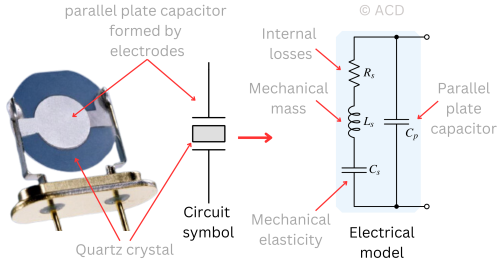
\includegraphics[width=0.7\linewidth]{images/Quartz Oscilator.png}
    \caption{Oscilador de Quartzo\cite{analog_oscillators_notes}.}
    \label{fig:Quartz Oscilator}
\end{figure}


O cristal de quartzo é um cristal Piezoelétrico, em verdade, foi o primeiro cristal dessa categoria descoberto \cite{mould_piezo}. Tais cristais, devido a sua estrutura molecular não centrocimétrica, isto é, com distribuição de cargas assimétricas, conduzem corrente quando deformados e são isolantes em estado de relaxamento \cite{mould_piezo}. Dado um potencial inicial, o cristal deforma, conduz corrente e depois oscila em sua frequencia de ressonancia natural \cite{mould_quartz}.

Entretanto, com o decorrer do tempo, a energia do sistema é dispersa e as oscilações do circuito ressonante diminuem em amplitude até que parem completamente no equilíbrio. Por isso, além do oscilador ressonante, é necessário um sistema de feedback e amplificação do sinal, para que esta oscilação seja mantida. 

\begin{figure}[H]
    \centering
    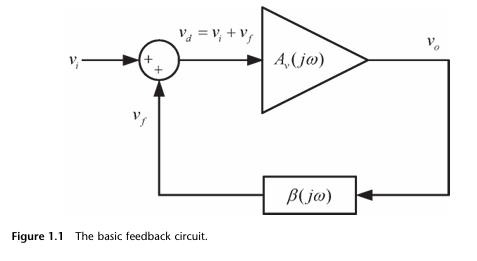
\includegraphics[width=0.6\linewidth]{images/oscilador-amplificador-feedback.png}
    \caption{Sistema de Feedback e Amplificação. \cite{gonzales2007}}
    \label{fig:oscilador-amplificador-feedback}
\end{figure}

No Logisim, esse circuito de oscilador será representado por este componente, nativo do simulador e com clock personável no próximo sistema.

\begin{figure}[H]
    \centering
    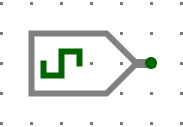
\includegraphics[width=0.2\linewidth]{images/clock-logisim.png}
    \caption{Clock no Logisim Evolution}
    \label{fig:clock-logisim}
\end{figure}
\subsection{Estrutura de um Clock de Redstone}

No contexto do Minecraft, o clock é implementado por meio de circuitos de redstone que exploram atrasos discretos introduzidos por componentes como repetidores.

Diferentemente de circuitos eletrônicos físicos, nos quais o tempo é contínuo e os atrasos são fenômenos analógicos, o tempo no jogo é explicitamente quantizado em \textit{ticks}, conforme definido anteriormente. Dessa forma, tanto a propagação de sinais quanto a atualização de estados ocorrem em múltiplos inteiros de Game Ticks (GT) ou Redstone Ticks (RT).

Neste projeto, será utilizado um loop de repetidores de redstone que introduzem um atraso $\tau$ cada, em Redstone Ticks, de forma qual um pulso percorre continuamente um caminho fechado. 

Como no jogo não existe dispersão de energia do sistema ressonante, o sinal permanece indefinidamente, produzindo uma oscilação periódica cujo período $T$ é determinado pela soma dos atrasos introduzidos ao longo do circuito. Dessa forma, para melhor controle do período, serão utilizados os repetidores do mod \textit{Wired Redstone}.

\begin{figure}[H]
    \centering
    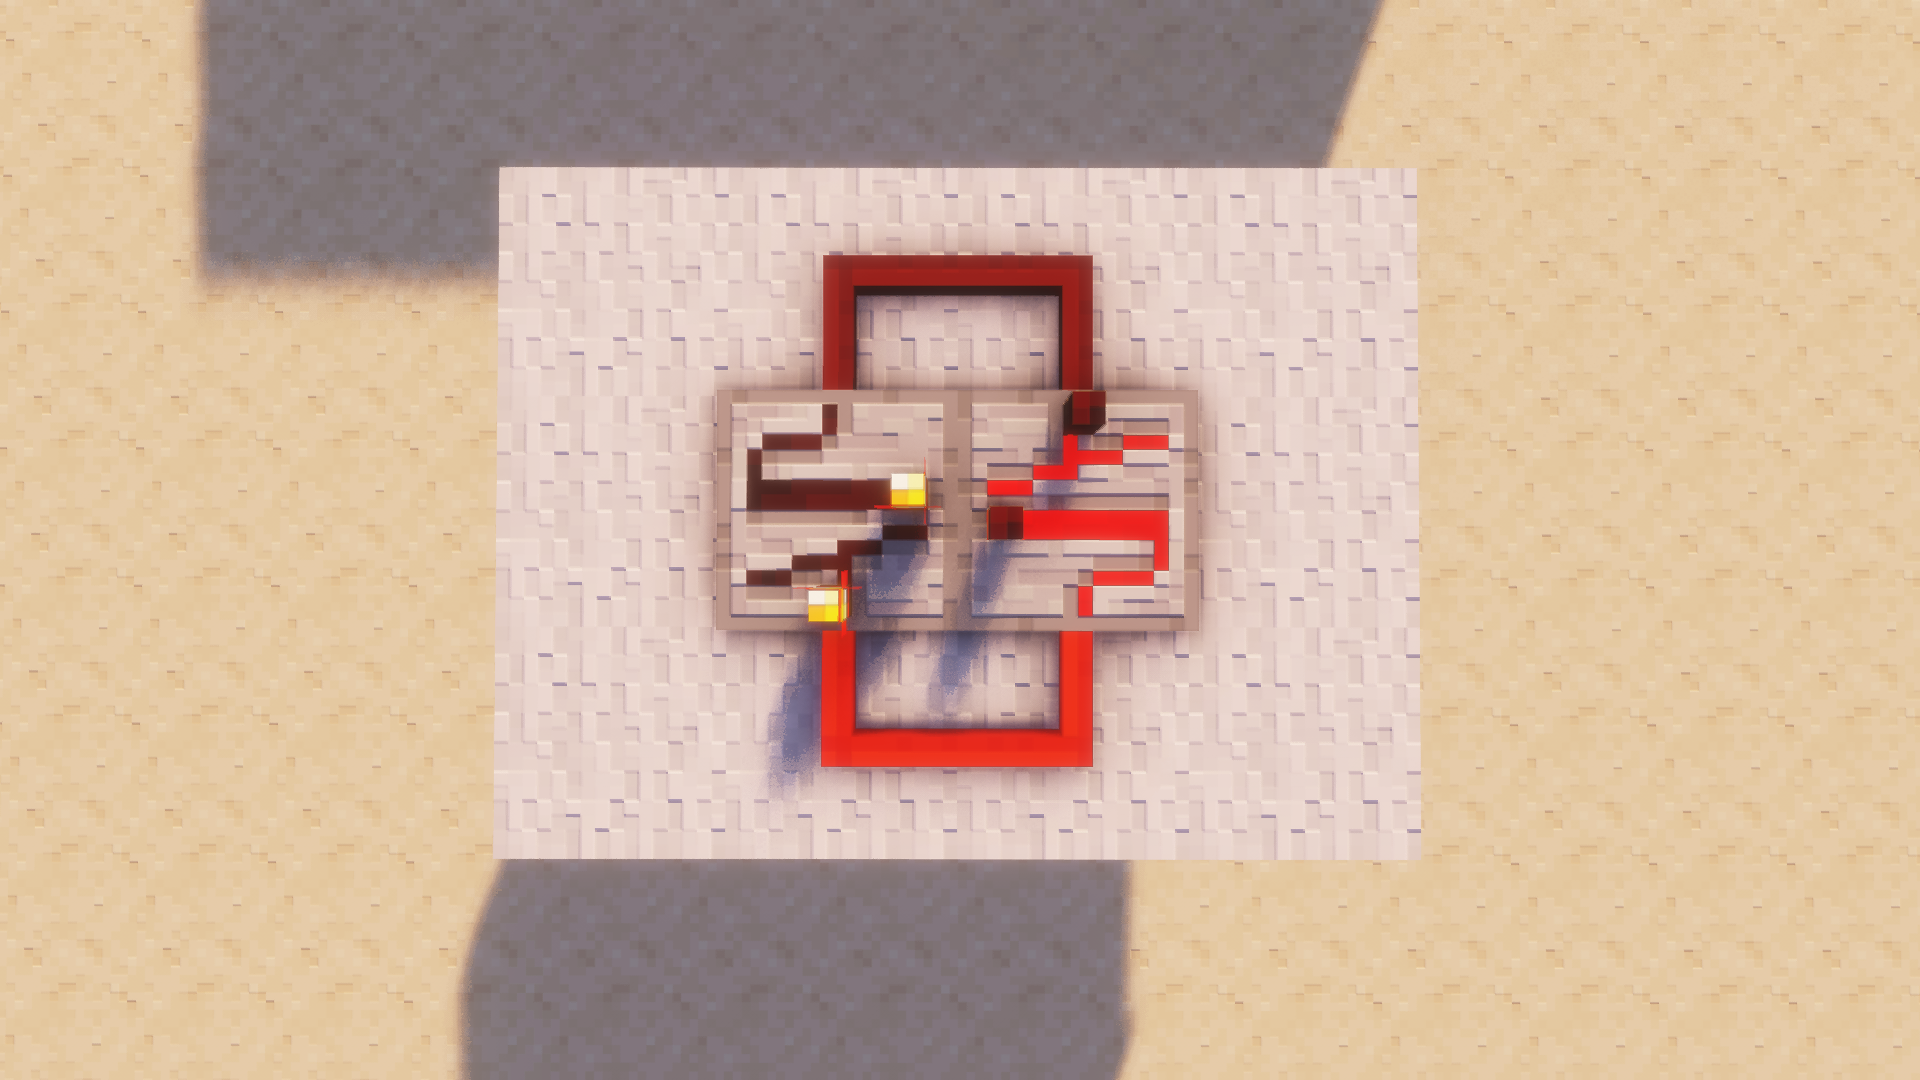
\includegraphics[width=0.7\linewidth]{images/clock-redstone.png}
    \caption{Clock no Minecraft}
    \label{fig:clock-redstone}
\end{figure}

Esta implementação, entretanto, possúi um problema central: não é possível desativar e reativar as oscilações. Portanto, um dos repetidores será substituido por uma porta AND, a qual introduz atraso $\alpha$ RTs, que receberá um bit $A$, de tal forma que para $A = 0$ o ciclo será aberto, atuando como um controlador/transistor/amplificador do sistema.  

\begin{figure}[H]
    \centering
    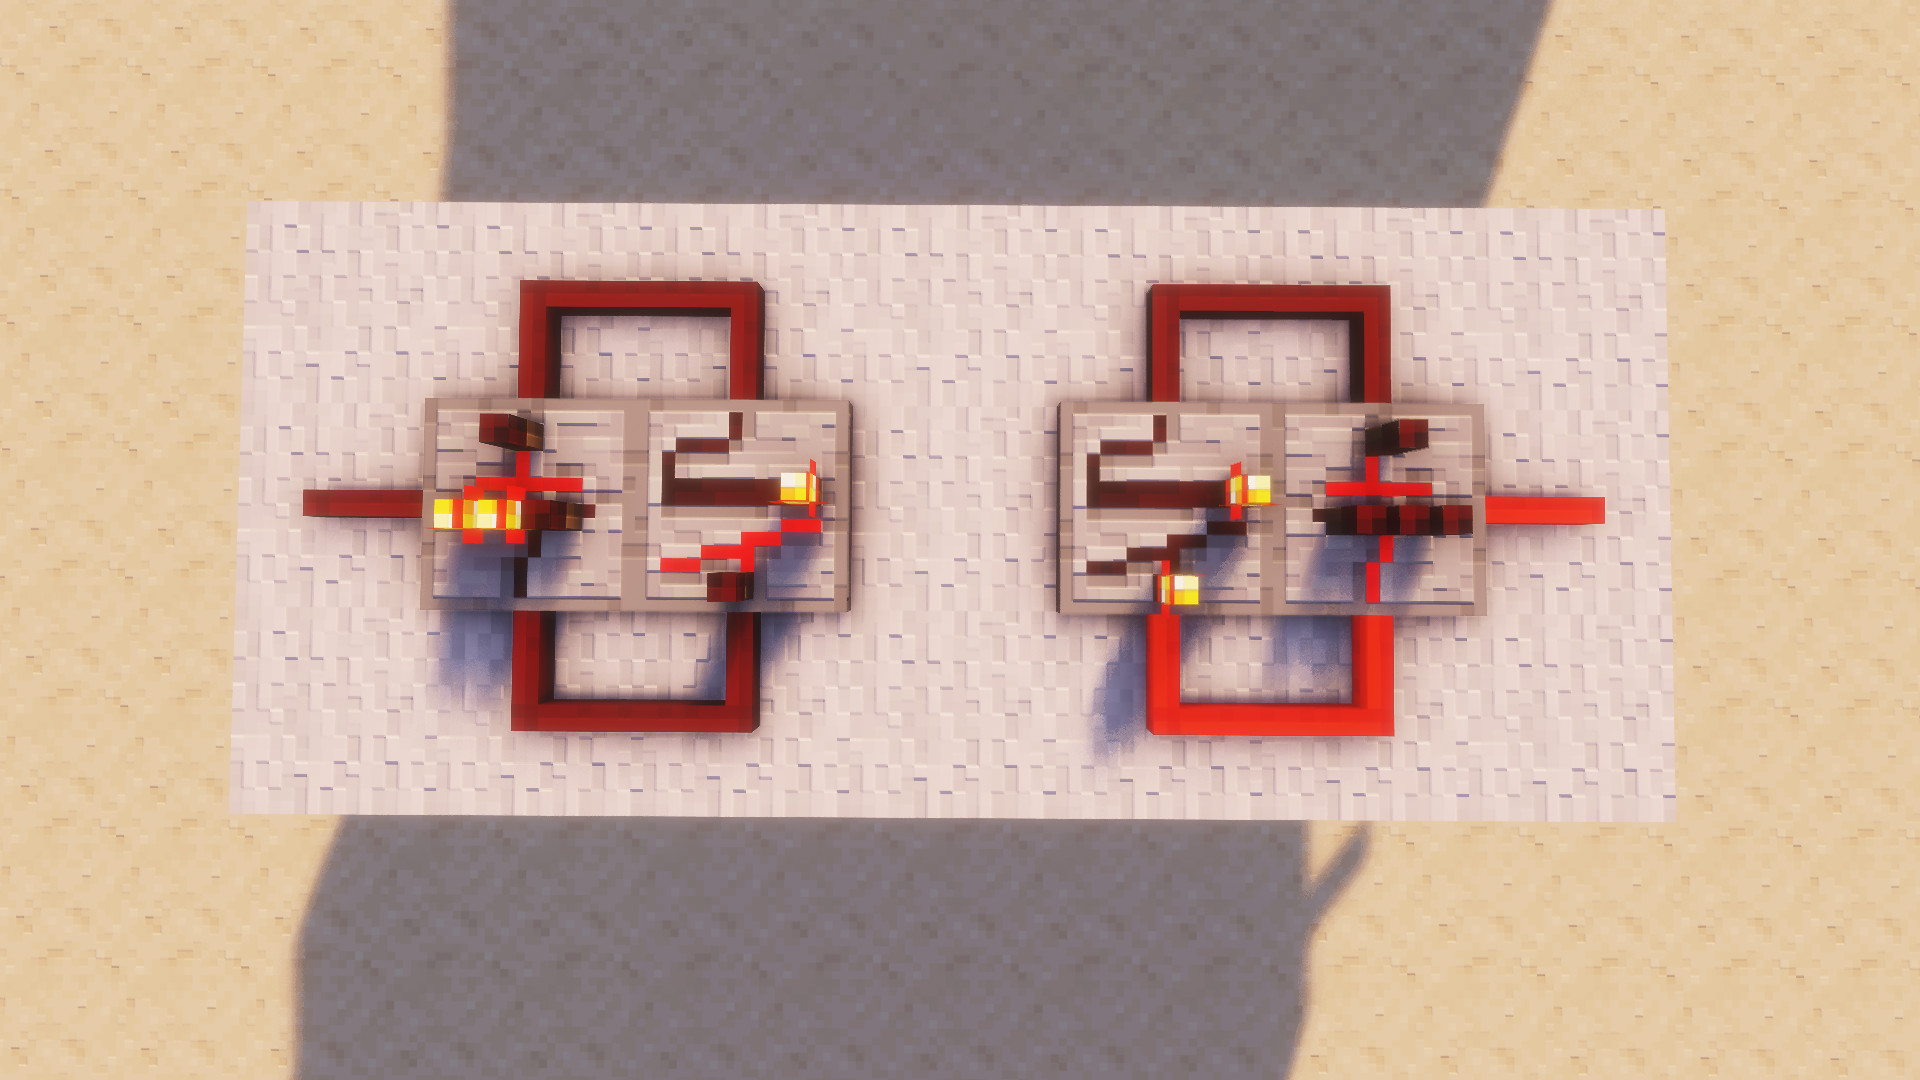
\includegraphics[width=0.7\linewidth]{images/clock-redstone-controlado.png}
    \caption{Clock no Minecraft com controle A}
    \label{fig:clock-redstone-controlado}
\end{figure}

A retomada das oscilações requer a injeção de um pulso inicial no circuito. Esse pulso atua como uma perturbação que passa a circular no loop, estabelecendo o regime periódico.

Para que o sistema opere corretamente, é necessário que exista apenas um único pulso propagando-se ao longo do circuito. Caso o pulso de ativação seja excessivamente longo, ele pode ocupar múltiplos estágios simultaneamente, resultando na formação de múltiplos pulsos no loop e, consequentemente, em comportamento incorreto do clock.

Seja $w$ a largura do pulso de ativação. Para garantir a propagação de um único pulso, deve-se impor a seguinte condição:

\[
w < \min(\tau, \alpha)
\]

onde $\tau$ representa o atraso dos repetidores e $\alpha$ o atraso introduzido pela porta de controle.

Essa restrição assegura que o pulso não se estenda por mais de um elemento do circuito ao mesmo tempo, preservando a integridade da oscilação periódica.
\subsection{Detecção de Bordas}

Em sistemas síncronos, as transições de estado ocorrem tipicamente nas bordas do sinal (subida ou descida), garantindo que todos os elementos de memória sejam atualizados de forma coordenada e evitando ambiguidades causadas por atrasos de propagação.

O detector de borda de subida identifica o momento em que um sinal transita de 0 para 1, gerando um pulso curto. Se este sinal for o clock ($clk$):

\begin{figure}[H]
    \centering
    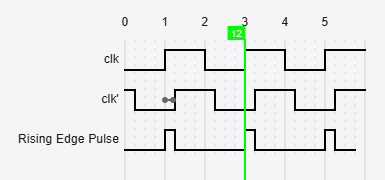
\includegraphics[width=0.7\linewidth]{images/rising-edge-detector-time-diagram.png}
    \caption{Timing digital do detector de borda de subida}
    \label{fig:rising-edge-detector-time-diagram}
\end{figure}

Esse comportamento pode ser descrito como:

\[
\text{Rising Edge} = clk \land \lnot clk_{delay}
\]

onde $clk_{delay}$ representa uma versão atrasada do sinal de clock, tal que $clk_{delay}(t) = clk(t - \Delta t)$.

Segue uma implementação do circuito de detecção de borda de subida: 

\begin{figure}[H]
    \centering
    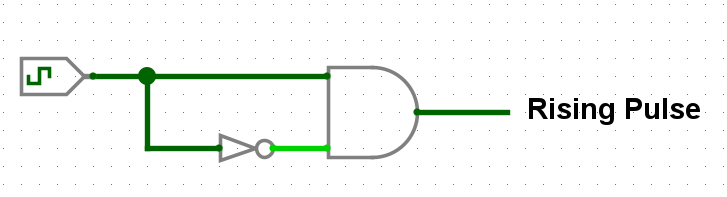
\includegraphics[width=0.7\linewidth]{images/rising-edge-detector.png}
    \caption{Detector de borda de subida}
    \label{fig:rising-edge-detector}
\end{figure}

O portão not introduz o delay $\Delta t$ ao mesmo tempo que respeita a equação acima.

\begin{figure}[H]
    \centering
    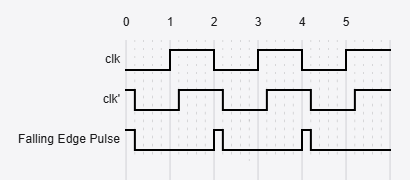
\includegraphics[width=0.7\linewidth]{images/falling-edge-detector-time-diagram.png}
    \caption{Timing digital do detector de borda de descida}
    \label{fig:falling-edge-detector-time-diagram}
\end{figure}

De forma análoga, o detector de borda de descida identifica a transição de 1 para 0:

\[
\text{Falling Edge} = \lnot clk \land clk_{delay}
\]

Uma implementação alternativa pode ser obtida a partir de uma transformação lógica utilizando as leis de De Morgan:

\[
\text{Falling Edge} = \lnot clk \land clk_{delay}
= \lnot (clk \lor \lnot clk_{delay})
\]

Essa forma é particularmente útil do ponto de vista de implementação, pois permite construir o detector utilizando uma porta NOR em conjunto com um inversor.

Nesse arranjo, o sinal $clk_{delay}$ é invertido e combinado com $clk$ por meio de uma porta NOR, produzindo diretamente o pulso correspondente à borda de descida.

Nesse caso, o pulso de saída é gerado no instante em que o sinal original já transitou para nível baixo, enquanto sua versão atrasada ainda permanece em nível alto, caracterizando a borda de descida.

\begin{figure}[H]
    \centering
    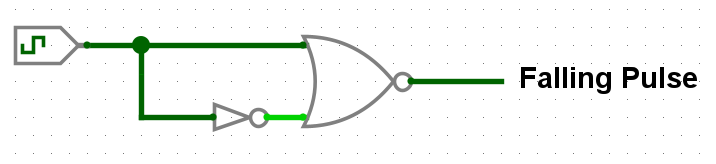
\includegraphics[width=0.7\linewidth]{images/falling-edge-detector.png}
    \caption{Detector de borda de descida}
    \label{fig:falling-edge-detector}
\end{figure}
\subsection{Considerações Práticas}

Embora o modelo apresentado seja conceitualmente simples, sua implementação prática depende diretamente do controle preciso do atraso $\Delta t$.

Para que o detector funcione corretamente, o atraso deve ser suficientemente pequeno para garantir que o pulso gerado seja curto, mas suficientemente grande para que exista uma diferença detectável entre $clk$ e $clk_{delay}$. Caso $\Delta t$ seja muito grande, o circuito pode gerar pulsos indesejados ou múltiplas ativações.

Além disso, variações no atraso de propagação dos componentes podem introduzir incertezas temporais, afetando a precisão da detecção de borda. Em sistemas reais, esse fenômeno está relacionado ao \textit{jitter} e ao \textit{skew} do clock.

Em ambientes discretos, como no Logisim ou em circuitos de Redstone, o atraso é quantizado, o que simplifica a análise, mas impõe limitações na resolução temporal do detector.

Apesar dessas restrições, detectores de borda são amplamente utilizados como mecanismos fundamentais para sincronização, sendo responsáveis por converter transições de nível em eventos discretos que podem ser utilizados por máquinas de estado e circuitos sequenciais.

Por exemplo, no Minecraft, para solucionar o problema do tamanho do pulso de retomada das oscilações, pode-se utilizar um detector de borda de subida no bit $A$. Dessa forma, quando ocorre uma transição $A_t = 0$ para $A_{t+1} = 1$. Tal pulso possui duração aproximadamente igual ao atraso $\Delta t$, garantindo que sua largura seja mínima e controlada, evitando a geração de múltiplos pulsos no circuito.

\begin{figure}[H]
    \centering
    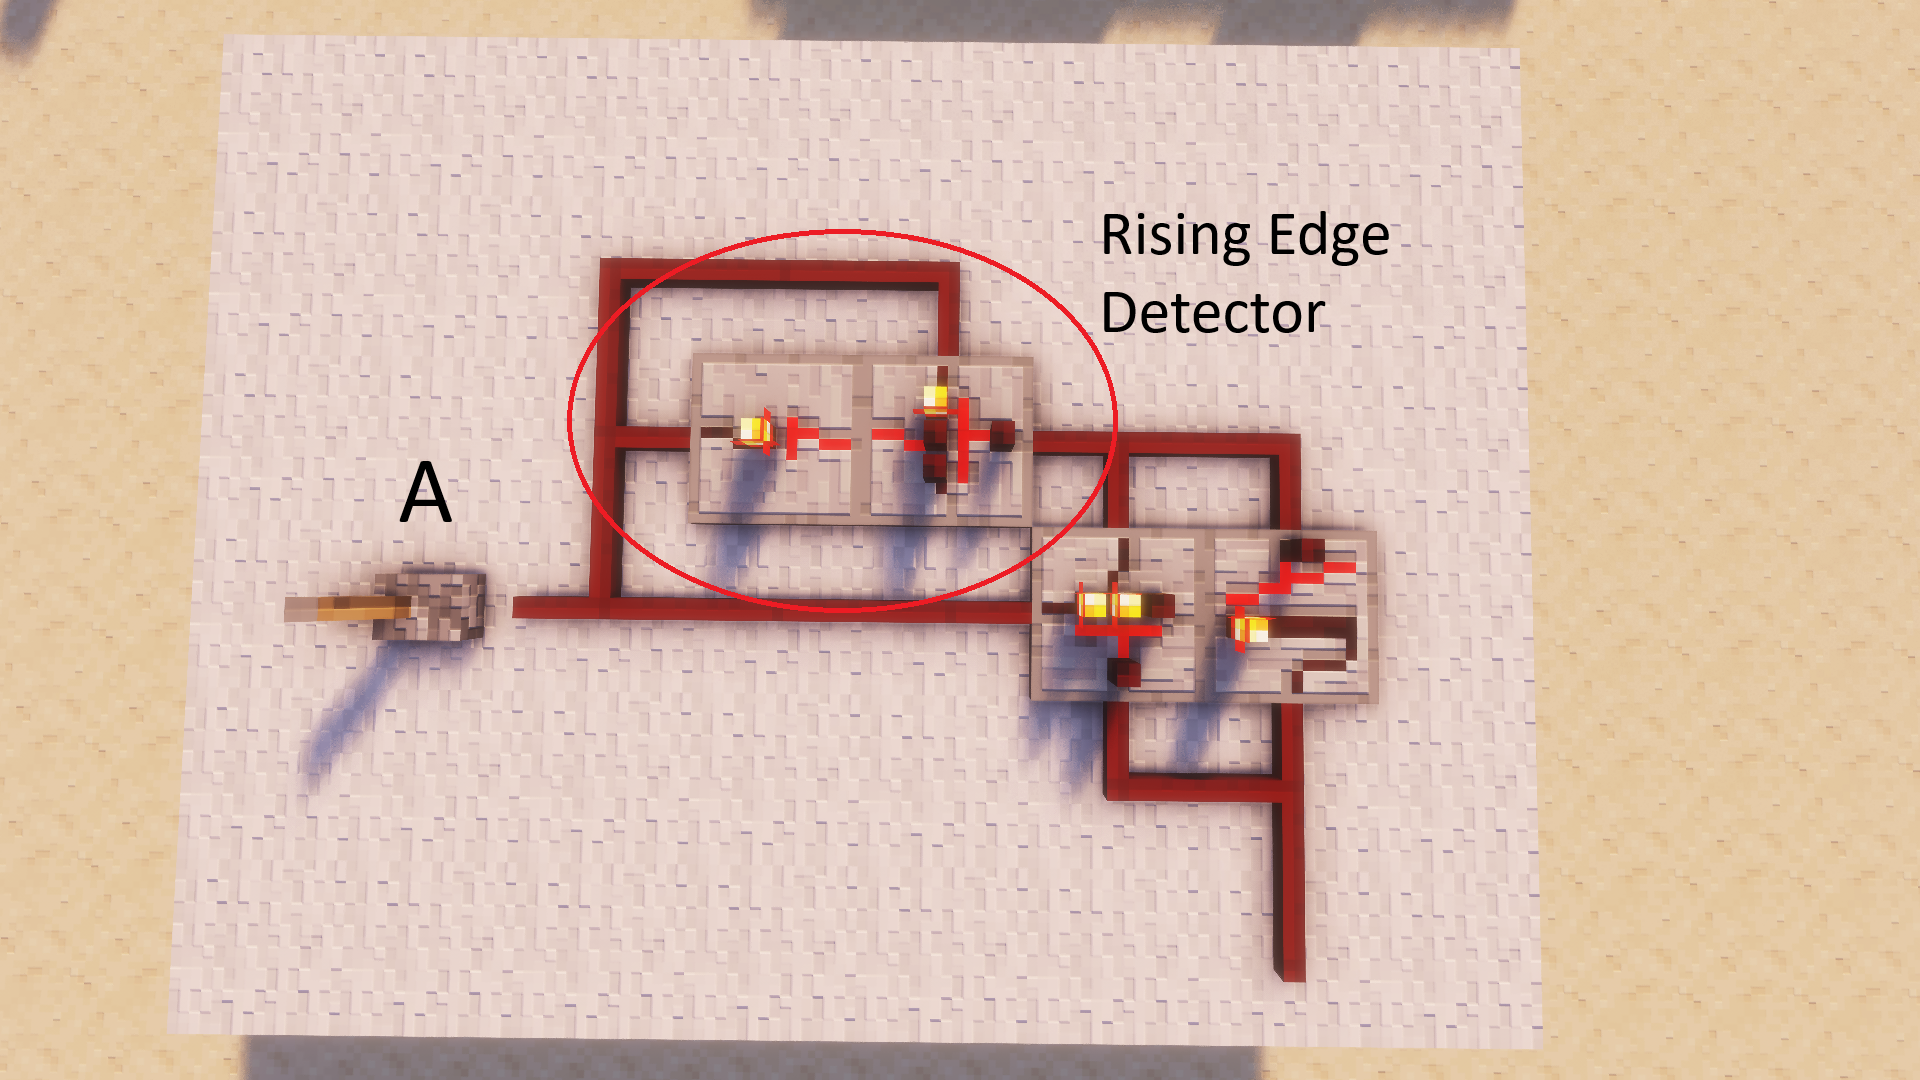
\includegraphics[width=0.8\linewidth]{images/toggle-redstone-clock.png}
    \caption{Clock on/of de redstone}
    \label{fig:toggle-redstone-clock}
\end{figure}

A título de curiosidade, existem tecnologias que exploram simultaneamente as bordas de subida e de descida do clock para realizar operações de leitura e escrita de dados. Essas tecnologias são conhecidas como \textit{Double Data Rate} (DDR).

Em sistemas DDR, os dados são transferidos duas vezes por período de clock: uma vez na borda de subida e outra na borda de descida. Dessa forma, para uma mesma frequência de clock $f$, obtém-se uma taxa efetiva de transferência equivalente a $2f$.

Essa abordagem permite aumentar o desempenho do sistema sem a necessidade de elevar a frequência do clock, o que é particularmente vantajoso devido às limitações físicas associadas a altas frequências, como maior consumo de energia, dissipação térmica e efeitos de propagação.
\subsection{Setup Time e Hold Time}

Para que elementos de memória, como flip-flops, que veremos na sessão \textbf{4.4}, operem corretamente, é necessário que suas entradas satisfaçam restrições temporais em relação ao sinal de clock.

\begin{figure}[H]
    \centering
    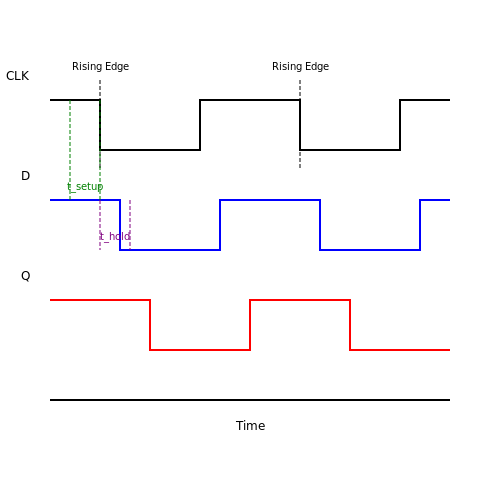
\includegraphics[width=0.7\linewidth]{images/setup-hold-times.png}
    \caption{Exemplo de setup e hold times para um Flip Flop tipo D}
    \label{fig:setup-hold-times}
\end{figure}

O \textit{setup time} ($t_{setup}$) é o intervalo mínimo antes da borda ativa do clock durante o qual a entrada deve permanecer estável.

O \textit{hold time} ($t_{hold}$) é o intervalo mínimo após a borda do clock durante o qual a entrada deve continuar estável.

Formalmente, se $t_0$ representa o instante da borda do clock, a entrada deve permanecer inalterada no intervalo:

\[
[t_0 - t_{setup},\ t_0 + t_{hold}]
\]

A violação dessas restrições pode levar a comportamentos incorretos.